\chapter{一元函数微分学}

\begin{introduction}
	\item 导数
	\item 微分
	\item 导数应用
	\item 微分中值定理
\end{introduction}

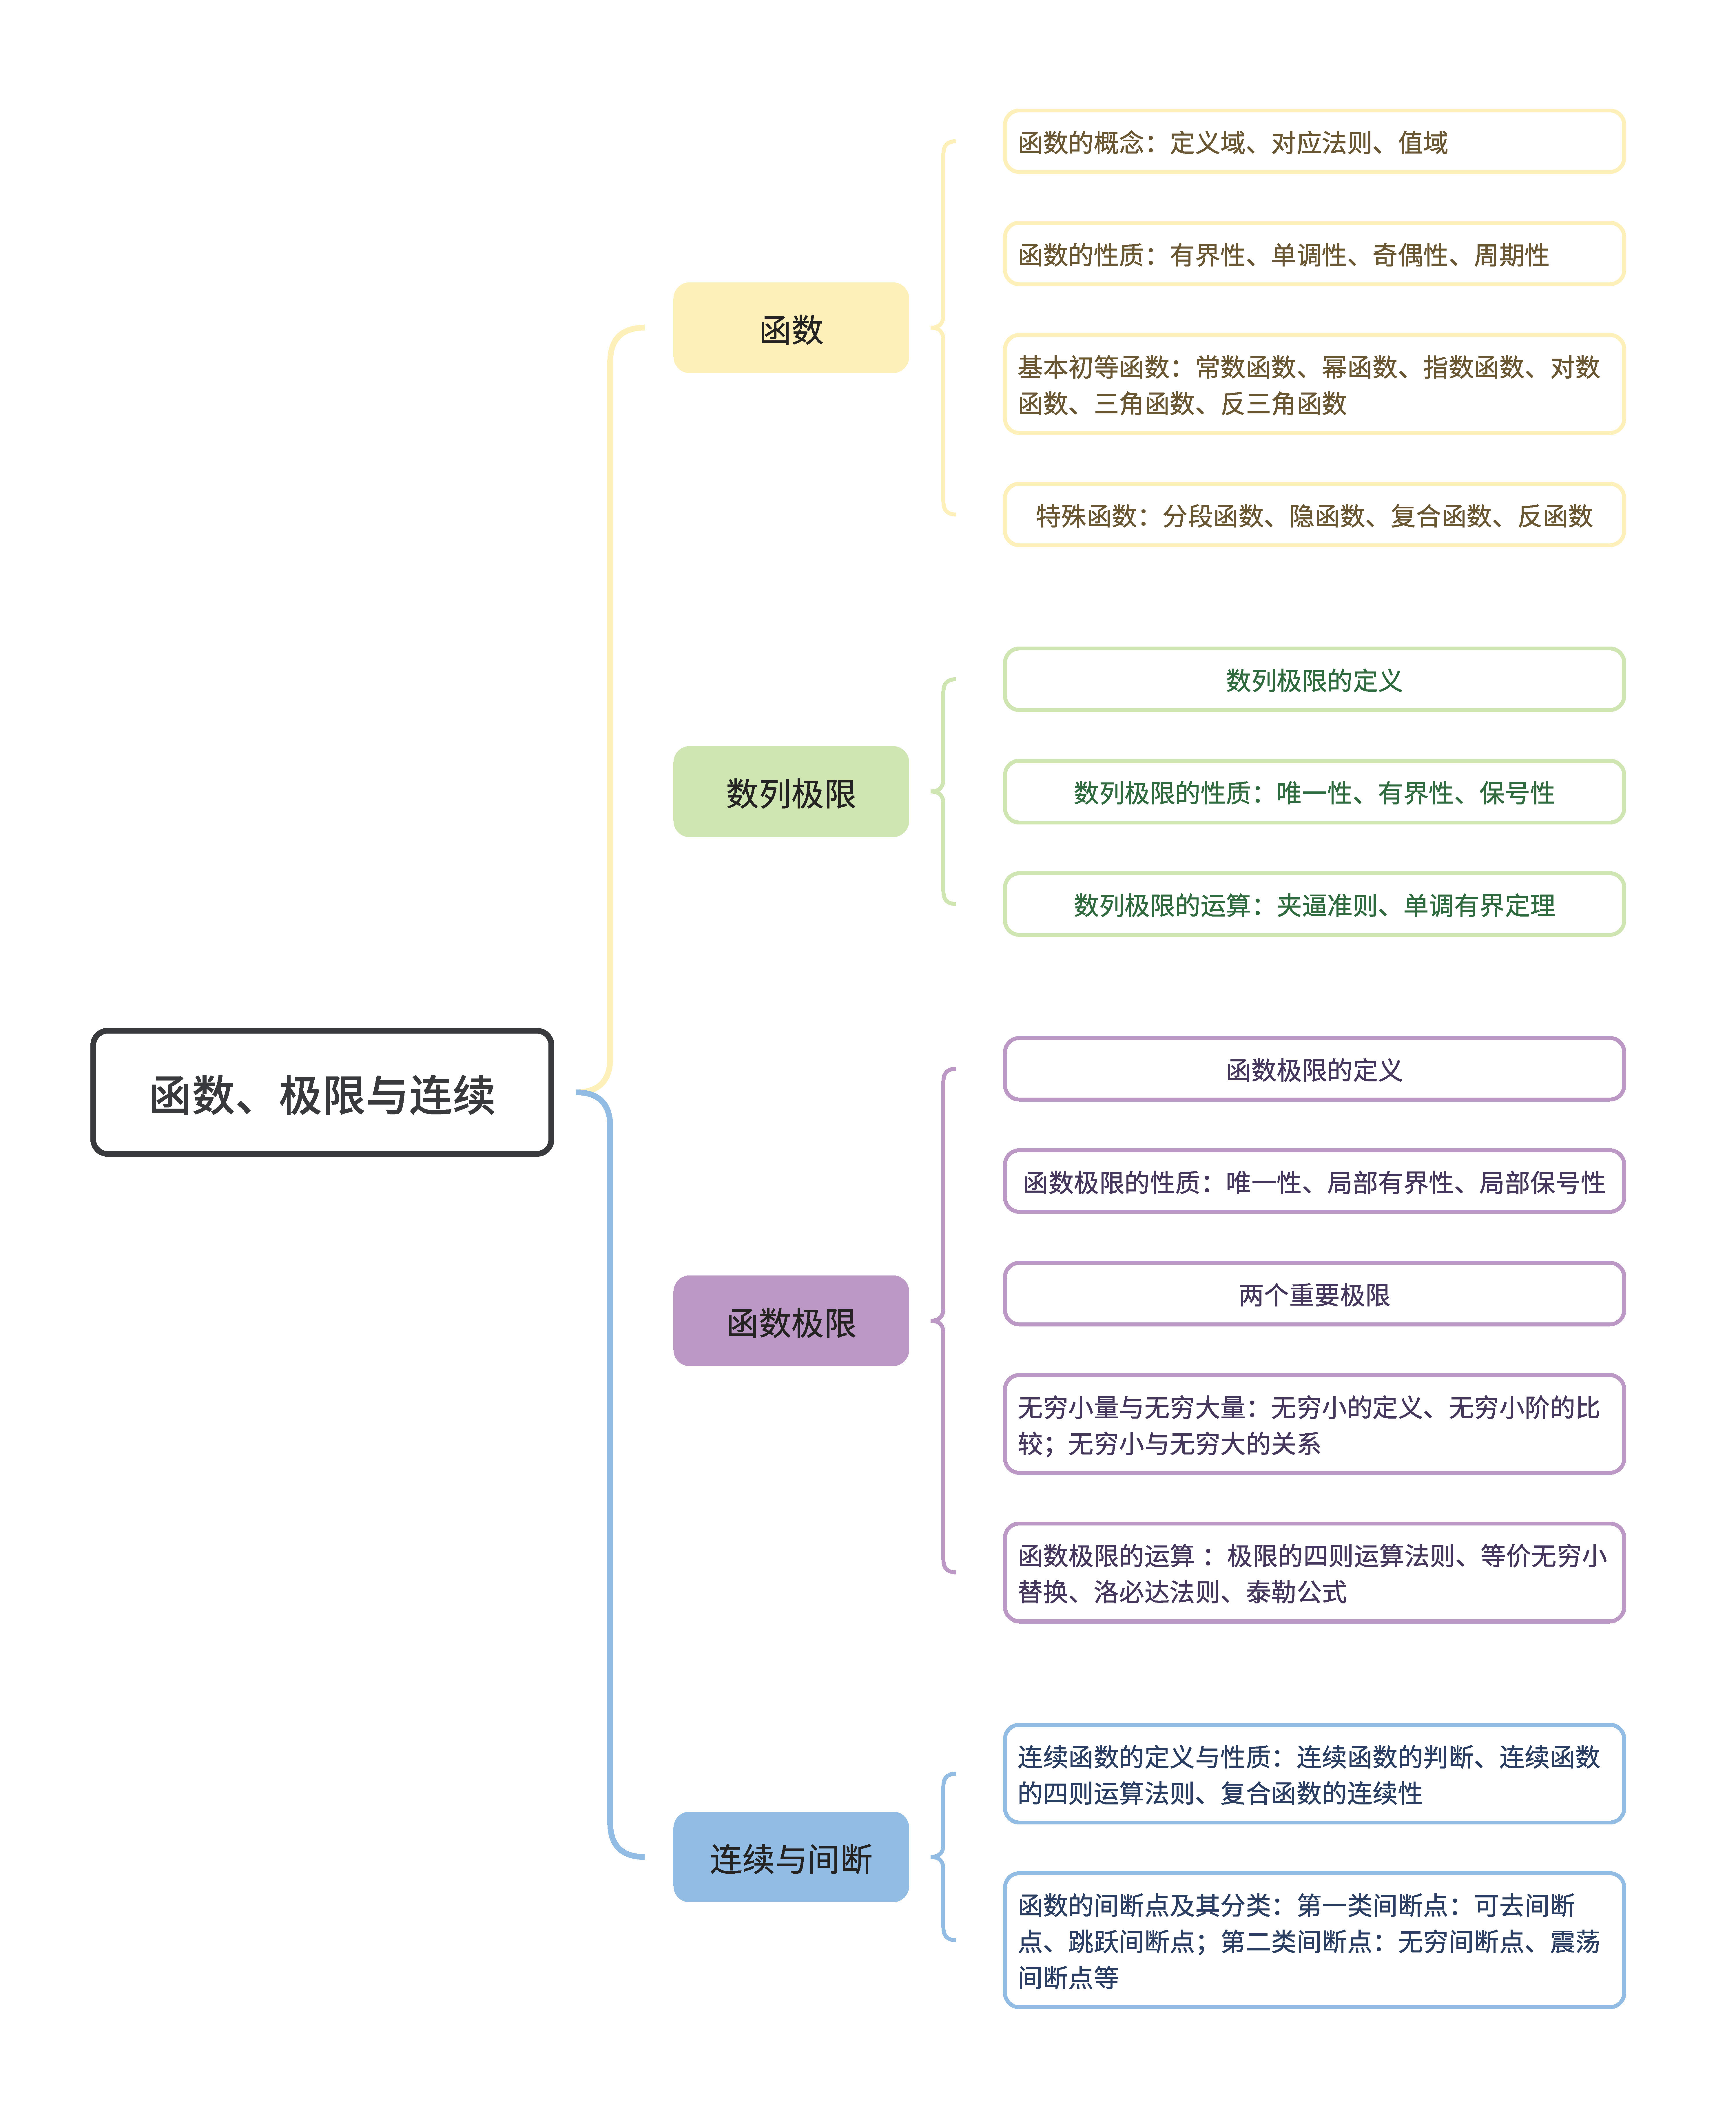
\includegraphics[width=6cm]{figure/chapter/chapter1.jpg}

\section{导数}
\subsection{导数的定义}
\subsection{导数的计算}



\section{微分}


\section{导数应用}
\subsection{函数的单调性}
\subsection{函数的极值与最值}
\subsection{函数的凹凸性与拐点}
\subsection{渐近线、曲率与曲率半径}


